%%%%%%%%%%%%%%%%%%%%%%%%%%%%%%%%%%%%%%%%%%%%%%%%%%%%%%%%%%%%%%%%%%%%%%%%%%%%%%%%%
% Diseño
%%%%%%%%%%%%%%%%%%%%%%%%%%%%%%%%%%%%%%%%%%%%%%%%%%%%%%%%%%%%%%%%%%%%%%%%%%%%%%%%%

\chapter{Diseño de la propuesta} % (fold)
\label{cha:Diseno}

    Aquí hay que detallar y justificar las decisiones que se tomen (hacer varias propuestas pero desarrollar solo la
    mejor) (siempre es bueno una tabla comparativa con pros y contras o ticks)

    \section{Librería de reproducción de sonido ¿?} % (fold)
    \label{sec:LibreriaDeReproduccionDeSonido}

        \begin{itemize}
            \item
            playsound\cite{playsound}: No se usa porque es muy lento y el programa que queremos crear necesita ser lo
            más rápido posible.
            \item
            mpg123\cite{mpg123}: Librería y programa en C más rápido que playsound de Python. Tiene el problema de
            hacer que haya fallos de memoria cuando se usan hebras para reproducir varios sonidos al mismo tiempo, pero
            se soluciona utilizando procesos en su lugar.
        \end{itemize}

    % section Librería de reproducción de sonido (end)

    \section{Otras librerías} % (fold)
    \label{sec:OtrasLibrerias}

        \begin{itemize}
            \item
            Wiring Pi\cite{wiringPi}: Para realizar la conexión de sensores y botones a la Raspberry Pi se utiliza
            la librería wiringPi, que es la estándar en este tema.
            \item
            pyserial\cite{pyserial}: Para realizar la conexión del Arduino a la Raspberry Pi, la salida que el Arduino
            escribe por la interfaz serial, se utiliza el módulo pySerial de Python.
        \end{itemize}

    % section Otras librerías (end)

    \section{Problemas ¿?} % (fold)
    \label{sec:Problemas}

        \begin{itemize}
            \item
            Error de \textit{segmentation fault} que ocurría por utilizar hebras para reproducir
            varios sonidos al mismo tiempo, se solucionó cambiando las hebras por procesos.
            \item
            Relacionado con el problema anterior, intentando reproducir dos sonidos al mismo tiempo, para reducir
            la posibilidad de que el usuario toque dos instrumentos al mismo tiempo. En el modelo solo por procesos
            se editan los sonidos juntos para que no haya latencia al tocar dos a la vez, haciéndolo con hebras se
            ahorra el trabajo de editar los sonidos y no hay combinaciones no contempladas. Sin embargo, el sistema
            de reproducción de sonido del sistema operativo no permite reproducir sonidos mediante hebras, solo
            procesos.
            \item
            En el prototipo con botones, al pulsar o dejar pulsado un botón, el programa reproduciría el mismo
            sonido muchas veces. Para solucionar esto se crea una hebra por cada botón, cuando se pulsa, entrará
            en un bucle infinito del que no saldrá hasta que el botón no sea soltado. Al usarse hebras, nos
            permite pulsar más botones al mismo tiempo.
            \item
            El sensor de presión devuelve muchas lecturas. Para solucionar esto a la hora de reproducir los sonidos
            hay dos formas de solucionarlo, una es introduciendo un \textit{delay} lo suficientemente grande para
            diferenciar dos toques del sensor, la otra solución, que ha sido la implementada, trata de bloquear el
            sensor cada vez que se entra en uno de los tres intervalos de volumen que se han elegido, cada vez que
            entra de deja de leer hasta que no baje la presión lo suficiente. Si la presión sube tampoco enviará
            señal para que reproduzca sonido.
            \item
            Al añadir el sensor y el Arduino, el programa que controlaba los sonidos emitidos recibía las mediciones
            del Arduino y, dependiendo de los datos entregados por éste, se emite un sonido a un volumen concreto.
            La construcción de la cadena de texto que contenía el \textit{path} se hacía mediante las funciones de
            copia y concatenación \textit{strcat} y \textit{strdup}. El problema es que al recibir el \textit{path},
            la biblioteca de reproducción de sonidos lanzaba el siguiente error:

            \begin{verbatim}
            malloc(): corrupted top size
            make: *** [Makefile:19: run] Segmentation fault
            \end{verbatim}

            Tras muchas pruebas, como aumentar la cantidad de memoria reservada para el \textit{path} o para el
            buffer que se utiliza en la función de reproducción, o probar a que siempre se enviara el mismo path,
            sin leer del Arduino (reproduciendo el sonido satisfactoriamente), finalmente decido cambiar la forma en
            la que se genera el path, \textit{hardcodeándolo} en el programa. Esto resulta funcionar y es la solución
            que ha sido implementada en el programa.
        \end{itemize}

    % section Problemas (end)

    \section{Sonido en paralelo} % (fold)
    \label{sec:SonidoEnParalelo}

        Hasta febrero, todas las versiones del programa fueron diseñadas pensando solo en emitir un sonido cada vez,
        pero lo preferible en un proyecto como este es que se emita más de un sonido al mismo tiempo.\newline

        El primer acercamiento fue mediante un sistema de máximos y sonidos combinados. En esta primera solución, se
        escogía el mayor de los seis sonidos y, si había un segundo sonido con un valor mayor que 200 (el mínimo para
        emitir sonido), se enviaba un mensaje a través del log de Arduino seleccionando un sonido combinado. Estos
        sonidos habían sido combinados previamente utilizando los sonidos ya presentes en el proyecto.\newline

        Finalmente, esta solución no funcionó correctamente (no se enviaba la señal del sonido combinado) y se procedió
        a diseñar una nueva. Esta nueva solución es la que se utiliza actualmente en el proyecto. Consiste en mandar
        todas las señales al mismo tiempo. Antes de la implementación de esta solución, el log era así:

        \begin{verbatim}
        0:0
        0:0
        2:364
        0:0
        0:0
        \end{verbatim}

        Tras la implementación de la solución, el log es así:

        \begin{verbatim}
        0:0
        0:0
        1:446:2:0:3:812:4:0:5:0
        0:0
        0:0
        1:0:2:0:3:0:4:902:5:0
        0:0
        \end{verbatim}

        En cuanto un sensor detecta una presión mayor a 200, se manda el mensaje de todos los sensores al mismo tiempo.
        En caso de que el valor leído sea menor que 200, se manda como 0, pero si es mayor, se manda con los demás. Este
        mensaje es leído y procesado por la Raspberry Pi, que lanzará los procesos necesarios con los sonidos que hagan
        falta según los sensores que hayan sido presionados.\newline

        Con esta segunda propuesta, el programa envía correctamente la señal de todos los sensores y los sonidos son
        emitidos correctamente.

    % section Sonido en paralelo (end)

    \section{Decisiones ¿?} % (fold)
    \label{sec:Decisiones}

        \subsection{if-else vs switch} % (fold)
        \label{sub:if-else_vs_switch}

            Al pulsar una tecla, el número leído se envía a una función que selecciona qué sonido hay que reproducir en
            ese momento, dependiendo de qué sonido corresponda a ese número. Este proceso de selección se puede hacer
            con una estructura de \textit{if-else} anidados o con un \textit{switch-case}.\newline

            Para decir cuál de las dos soluciones se implementa en la versión final se realizó un test en el que cada
            vez se ejecutan más iteraciones del programa cambiando de sonido en cada una de ellas. Se empieza con 1
            iteración y se termina con 10000000 iteraciones.\newline

            \begin{figure}[ht]
                \centering
                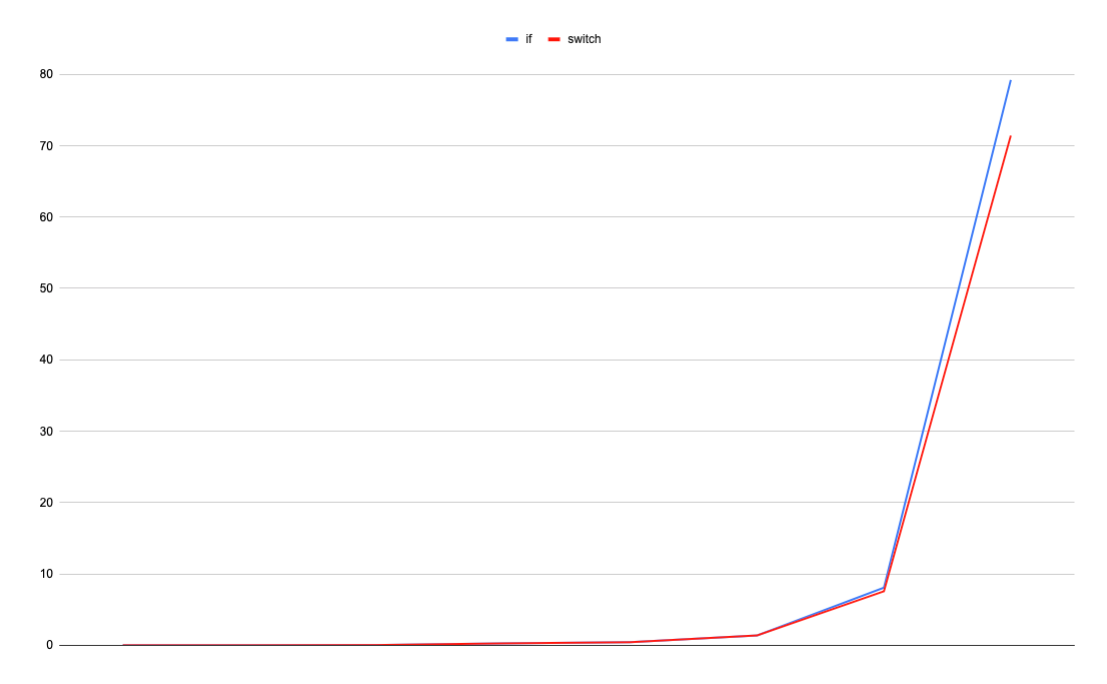
\includegraphics[width=\textwidth]{grafica_if_switch}
                \caption{Gráfica comparativa if-else vs switch}
            \end{figure}
            \begin{center}
                \begin{tabular}{ |c|c|c| }
                    \hline
                        iterations & if & switch \\
                        \hline\hline
                        1 & 0.000243 & 0.000270 \\
                        \hline
                        10 & 0.002797 & 0.002485 \\
                        \hline
                        100 & 0.027775 & 0.027261 \\
                        \hline
                        1000 & 0.260075 & 0.261464 \\
                        \hline
                        10000 & 0.431544 & 0.425668 \\
                        \hline
                        100000 & 1.368561 & 1.374575 \\
                        \hline
                        1000000 & 8.070825 & 7.560718 \\
                        \hline
                        10000000 & 79.199539 & 71.409653 \\
                    \hline
                \end{tabular}
            \end{center}

            Como se puede ver en la gráfica, la diferencia no es apreciable hasta las 1000000 iteraciones, pero después
            pasa a casi 8 segundos de diferencia en 10000000 iteraciones. Por esta razón se ha decidido que la función
            utilice la estructura \textit{switch-case}.\newline

            Finalmente, debido a la manera en la que realizan las comprobaciones de qué botones y sensores son
            utilizados, aunque un \textit{switch-case} es más rápido, esta estructura se reserva para la versión del
            programa que reproduce los sonidos leyendo del teclado. En el programa que controla los sensores se utiliza
            una estructura \textit{if-else}.

        % subsection if-else vs switch (end)

    % section Decisiones (end)

    \subsection{Arduino} % (fold)
    \label{sub:Arduino}

        Para la recepción de las señales del sensor de presión RP c18.3, se plantean dos opciones, se puede utilizar
        la propia Raspberry Pi en la que se ejecuta el programa que maneja los sonidos o una Arduino Nano. En el
        proyecto resultante se utiliza finalmente la Arduino debido a dos razones principales.\newline

        La primera razón es el precio y la escalabilidad, una Raspberry Pi cuesta 39,95\euro{} mientras que una
        Arduino Nano cuesta 10\euro{}. Una Arduino Nano cuenta con menos pines de E/S, pero añadir una placa es más
        barato y sencillo que añadir una placa de Raspberry Pi.\newline

        La segunda razón es la implementación del programa que se encarga de el sensor de presión. En Internet se
        pueden encontrar ejemplos y tutoriales refiriéndose a cómo implementar el sistema en una Arduino, pero no
        es tan fácil encontrar información para hacerlo desde una Raspberry Pi.\newline

        Por estas razones se elige realizar la recepción de las señales del sensor de presión desde la Arduino,
        haciendo el proceso más sencillo y más barato.

    % subsection Arduino (end)

% chapter Diseño (end)